\chapter{Tools and technologies}
\label{chapter5}

In this chapter, we will thoroughly describe the tools, technologies and other materials that were utilized in any way to help in the development of this Degree Final Project. This includes any necessary programming languages, plugins, IDEs, APIs, database engines, data sources and any other software development and documentation tools that were needed at any stage of the process for building the mobile application.

Besides, for some of them we will also provide a comparison with other similar options and justify why it was finally decided to choose them for this project over the rest of available solutions. As a summary, the tools and technologies that were used to plan and develop the mobile application are the following:

\begin{itemize}
\item During the preprocessing of the input images, use will be made of the OpenCV \cite{noauthor_opencv_2021} library for artificial vision, open source and available for Python \cite{noauthor_python_2021} through OpenCV-Python \cite{noauthor_opencv-python_2021}.
\item To capture the text, we will work with the Tesseract \cite{noauthor_tesseract_2021} optical character recognition engine, also open source, and with the Python-tesseract wrapper \cite{lee_pytesseract_2021}.
\item In the case of post-processing the text and obtaining the list of ingredients, use will be made of the library of tools for natural language processing NLTK \cite{noauthor_natural_2021}.
\item The database will be created and maintained using the MySQL relational management system \cite{noauthor_mysql_2021}.
\item The application for Android devices will be implemented using the Flutter software development kit \cite{noauthor_flutter_2021}.
\item The development of all the code will be done using the Visual Studio Code text editor \cite{noauthor_documentation_2021}, as well as the Android Studio IDE \cite{noauthor_introduccion_2021}. The source code control will be done with Git \cite{noauthor_git_2021} and GitHub \cite{noauthor_githubcom_2021}.
\end{itemize}

\section{Framework}

In this section we will introduce and discuss the framework chosen to support the mobile application architecture, Flutter, going though some of its main characteristics. We will also detail the programming language it uses, Dart, as well as the most relevant Flutter plugins that were utilized during development.

\subsection{Flutter}

Flutter \cite{noauthor_flutter_2021} is an open-source framework for mobile applications development created by Google in 2017. It supports cross-platform development, allowing to generate Android, iOS and web apps from the same codebase. Its logotype is shown in Figure \ref{fig:flutter}.

\begin{figure}[h]
  \centering
  
\includegraphics[width=0.5\textwidth]{Figures/flutter.png}
  \caption{%
    Flutter's logotype
  }
  \label{fig:flutter}
\end{figure}

Its main characteristic is that all of the app design and architecture in Flutter is based on components called widgets. A widget in Flutter can be any description of part of a user infer face along with some data. We can combine several simple widgets to produce more complex ones, thus organizing all the interface design and behaviour in a hierarchical tree structure where every element is a widget. In Figure \ref{fig:flutter-widgets} we can see an example of this tree hierarchy for a simple app.

\begin{figure}[h]
  \centering
  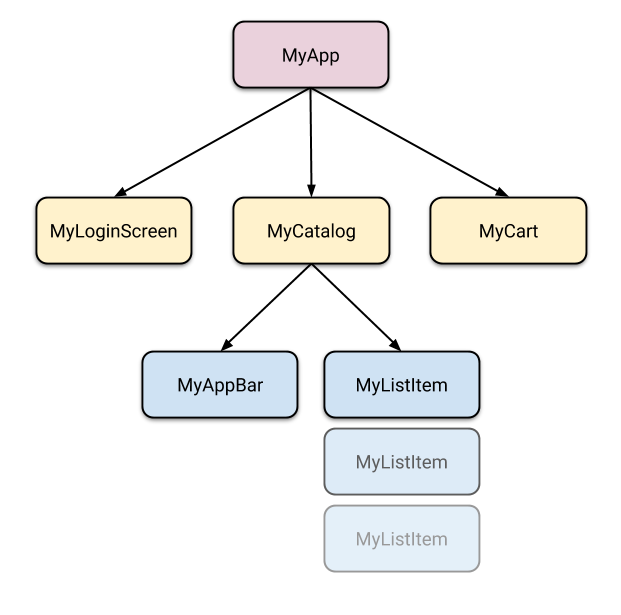
\includegraphics[width=0.5\textwidth]{Figures/flutter-widgets.png}
  \caption{%
    Tree of widgets that compose a Flutter app
  }
  \label{fig:flutter-widgets}
\end{figure}

Some of these widgets are already predesigned to conform to established design guidelines, such as Material Design \cite{noauthor_material_nodate} for Android or the Cupertino library for adhering to iOS style. In our application, we made extensive use of the Material library in order to keep a consistent design with other Android apps.

These support for visually clean components gave it an edge over other similar frameworks available for cross-platform development, such as React Native, Xamarin or Ionic. Other reasons for choosing Flutter are that its developed by the same company that maintains Android, Google, and that the community built around Flutter has gotten quite large over the recent years. In fact, during the development of this project, we managed to locate and solve several issues by contacting other Flutter developers via channels like GitHub or Discord.

An example of this communications can be seen in Figure \ref{fig:flutter-issue}, which shows an issue opened to fix a camera bug.

\begin{figure}[h]
  \centering
  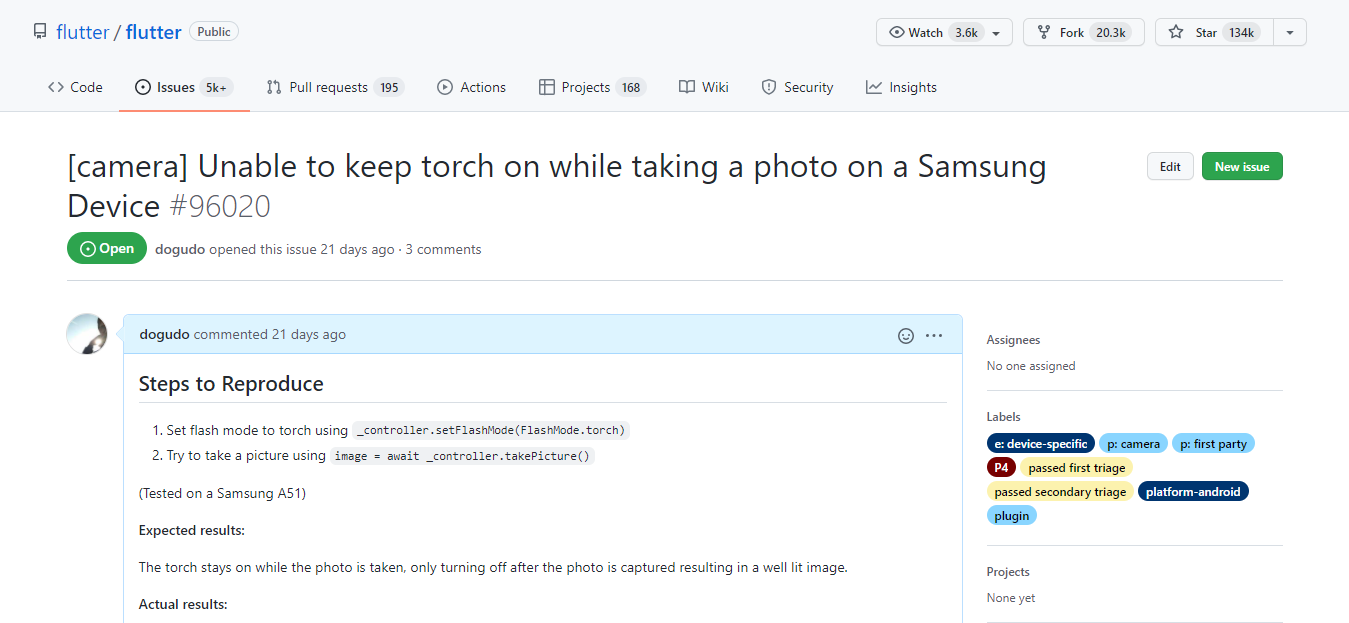
\includegraphics[width=\textwidth]{Figures/flutter-issue.png}
  \caption{%
    Issue opened in Flutter's issue tracker
  }
  \label{fig:flutter-issue}
\end{figure}

Lastly, the programming language that is utilized through all stages of Flutter's app development is Dart.

\subsection{Dart}

Dart \cite{noauthor_dart_nodate-1} is an open-source programming language developed by Google and specifically designed for web and mobile apps development. As it has been mentioned, it is Flutter's development language although it was first released in 2010. It is optimized for client-side development and one of its biggest strengths is capability to compile to either native code or JavaScript. This way, it is properly suited for cross-platform development. Its logotype can be seen in Figure \ref{fig:dart}.

\begin{figure}[h]
  \centering
  
\includegraphics[width=0.5\textwidth]{Figures/dart.png}
  \caption{%
    Dart's logotype
  }
  \label{fig:dart}
\end{figure}

Some of Dart's most relevant and differentiating characteristics from other languages are listed below:

\begin{itemize}
\item \textbf{Null safety}: by default, values in Dart cannot be null unless the developer explicitly specifies so.
\item \textbf{Strongly typed}: although type annotations are optional because they can be inferred by the compiler.
\item \textbf{Asynchronous programming}: supported by using futures as well as the \texttt{async} and \texttt{await} keywords. This is specially useful for interfaces, where some elements may need to wait for some other operation to finish before being displayed.
\end{itemize}

For quick reference of how a Dart code file actually looks like, a snippet from the application is provided on Listing \ref{lst:dart}.

\begin{code}
\begin{minted}
[
breaklines,
frame=lines,
framesep=2mm,
baselinestretch=1.2,
fontsize=\footnotesize,
linenos
]
{dart}
  Widget build(BuildContext context) {
    return AnnotatedRegion<SystemUiOverlayStyle>(
      child: Scaffold(
        appBar: AppBar(
          title: Text(widget.title),
          systemOverlayStyle: const SystemUiOverlayStyle(
            statusBarColor: Colors.transparent,
          ),
        ),
        body: Center(
          child: screens.elementAt(_selectedIndex),
        ),
        bottomNavigationBar: BottomNavigationBar(
          items: const <BottomNavigationBarItem>[
            BottomNavigationBarItem(
              icon: Icon(Icons.history),
              label: 'History',
            ),
            BottomNavigationBarItem(
              icon: Icon(Icons.home),
              label: 'Allergens',
            ),
          ],
          currentIndex: _selectedIndex,
          onTap: _onItemTapped,
        ),
      ),
    );
  }
\end{minted}
\caption{Example of Dart code}
\label{lst:dart}
\end{code}

\subsection{Plugins}

Flutter plugins or packages are libraries of code that expand the capabilities of the base framework. They are published in the package repository Pub \cite{noauthor_dart_nodate}, where developers can browse through a large collection of packages to easily incorporate other technologies, functionalities or APIs into their application. This repository's main page is seen in Figure \ref{fig:pub}.

\begin{figure}[h]
  \centering
  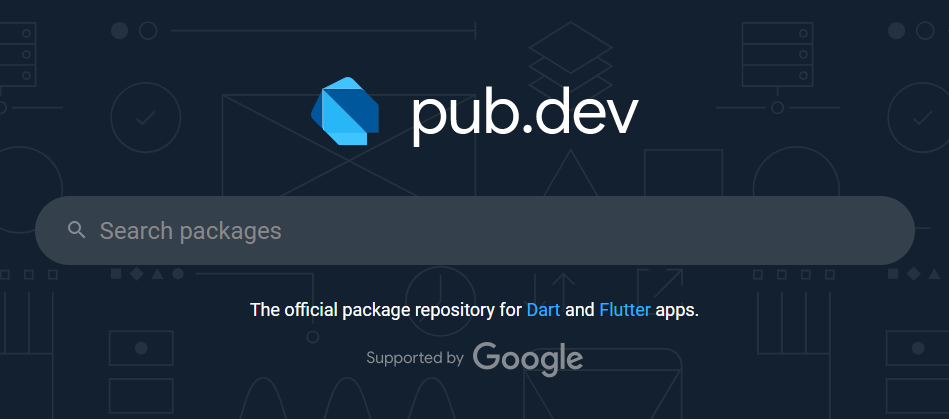
\includegraphics[width=0.75\textwidth]{Figures/pub.png}
  \caption{%
    Pub's homepage snippet
  }
  \label{fig:pub}
\end{figure}

In the development of our application we had to incorporate up to seven new dependencies into our codebase. Some of the most interesting ones are listed below:

\begin{itemize}
\item \textbf{\texttt{google\_ml\_kit}} \cite{noauthor_google_ml_kit_nodate}: recently released plugin that provides an easy way to implement Google's standalone ML Kit in a Flutter app instead of on a native Android one. It will be broadly discussed on the next section.
\item \textbf{\texttt{camera}} \cite{noauthor_camera_nodate}: a plugin providing access and some control functionality over the device cameras. Used for a better integration with our UI than when using the device native camera app.
\item \textbf{\texttt{sqflite}} \cite{noauthor_sqflite_nodate}: a plugin providing support for operating the SQLite database engine through a Flutter app.
\item \textbf{\texttt{http}} \cite{noauthor_http_nodate}: a future-based library dedicated to make HTTP requests, used mainly for API requests.
\end{itemize}

\section{SDK and API}

This section will further explain two of the main technologies at the core of the mobile application, its text recognition system and its translation system, and justify the choice of these solutions.

\subsection{Google ML Kit}

Google Ml Kit \cite{noauthor_ml_nodate} is a mobile SDK that provides on-device machine learning solutions to both Android and iOS apps. By default, only native Android apps are supported by this SDK. However, by using the \texttt{google\_ml\_kit} plugin previously mentioned, it is considerably simpler to make use of this technology on a Flutter application.

Even though initially this technology did not support Korean language for its text recognition models, support for non-Latin scripts like \textit{hangeul} among others was added on a beta update released on August of 2021. This allows for accurate Korean text recognition without needing to incur on external API additional costs, since all the processing is done on-device. On the downside, the size of the application increases considerably, up to 400 MB.

In addition to this text recognition API, an on-device translation API is also provided. Due to its low accuracy this one is used only as a fallback for when the main one, the Papago API, is not available.

\subsection{Papago API}

\section{Database}

\section{Development}

In this section, we will discuss mainly about the two different IDEs used during the programming and development of the mobile application: Visual Studio Code and Android Studio.

\subsection{Visual Studio Code}

Visual Studio Code \cite{noauthor_documentation_2021}, abbreviated as VS Code, is a code editor developed by Microsoft. It is free, open-source, and since its release in 2015 it has quickly risen to become the most popular source code editor by a great margin \cite{noauthor_stack_nodate}. It is highly customisable, with a library of plugins that provides support for virtually any programming language available. Figure \ref{fig:vscode-logo} depicts Visual Studio Code's logotype.

\begin{figure}[h]
  \centering
  
\includegraphics[width=0.25\textwidth]{Figures/vscode-logo.png}
  \caption{%
    Visual Studio Code's logotype
  }
  \label{fig:vscode-logo}
\end{figure}

Visual Studio Code is one of the two IDEs (along with Android Studio) that is officially supported for Flutter development, with a plugin that adds most of the functionality built in Android Studio such as hot-reload, support for Dart and several other coding and debugging options. Because of its simplicity, high modularity, widespread usage and complete support for Flutter, it was chosen as the text editor of preference during most of the development. We can see an screenshot of Visual Studio Code's interface in Figure \ref{fig:vscode-screen}.

\begin{figure}[h]
  \centering
  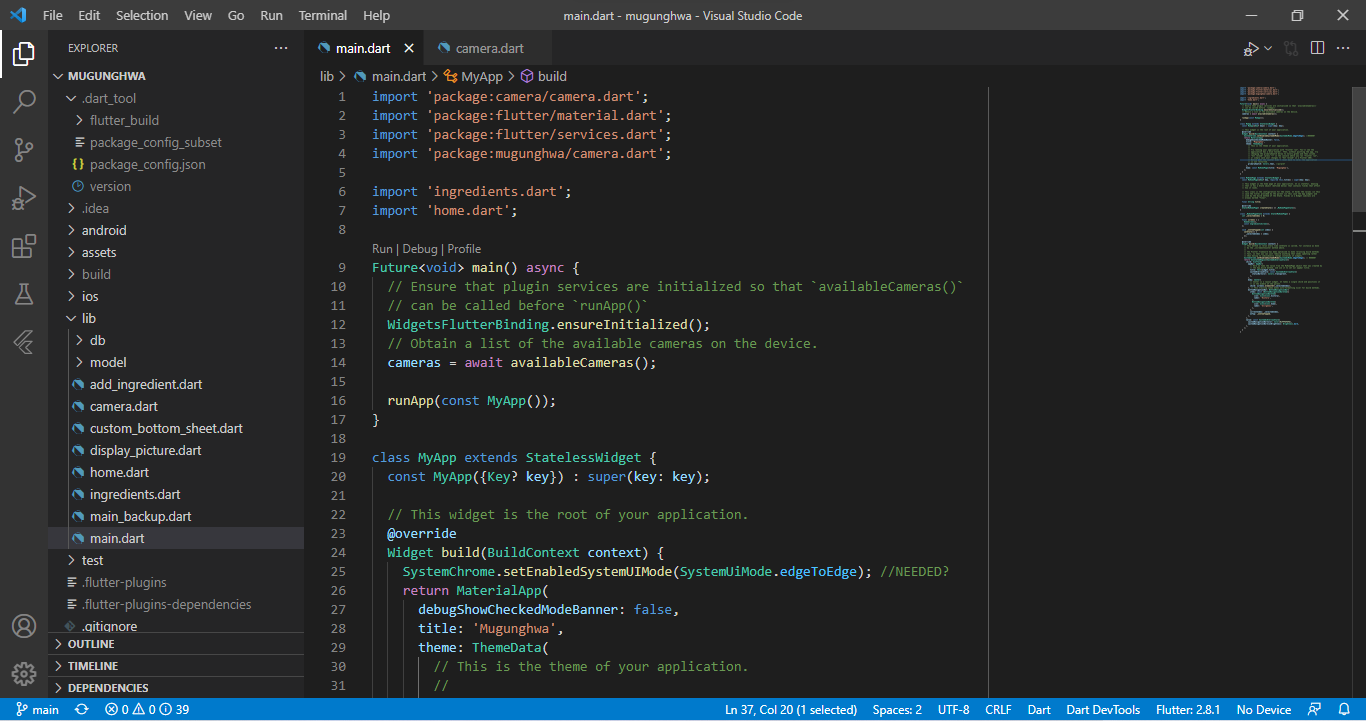
\includegraphics[width=\textwidth]{Figures/vscode-screen.png}
  \caption{%
    Visual Studio Code's user interface
  }
  \label{fig:vscode-screen}
\end{figure}

It is worth noting that Visual Studio Code also implements out-of-the-box support for version control systems such as Git. This way, we can commit, pull or push changes to our repository directly from VS Code interface without having to deal with a separate CLI interface.

\subsection{Android Studio}

Android Studio \cite{noauthor_introduccion_2021} is the official IDE for the Android platform, and therefore is also developed and maintained by Google. It was released in 2014 and replaced Eclipse as the standard IDE for Android app development. Though it natively only supports Java, Kotlin and C++, Dart support as well as most of the needed Flutter functionality can be added through the Flutter official plugin. Its logotype is shown in Figure \ref{fig:android-studio}.

\begin{figure}[h]
  \centering
  
\includegraphics[width=0.5\textwidth]{Figures/android-studio.png}
  \caption{%
    Android Studio's logotype
  }
  \label{fig:android-studio}
\end{figure}

Despite it being the default IDE for Android, Android Studio was only used during the initial stages of this project. This is due to it being way more heavy on resources than Visual Studio Code, making it more time inefficient for its usage on a machine with limited resources like the one used during development. Figure \ref{fig:android-studio-screen} shows the user interface of Android Studio.

\begin{figure}[h]
  \centering
  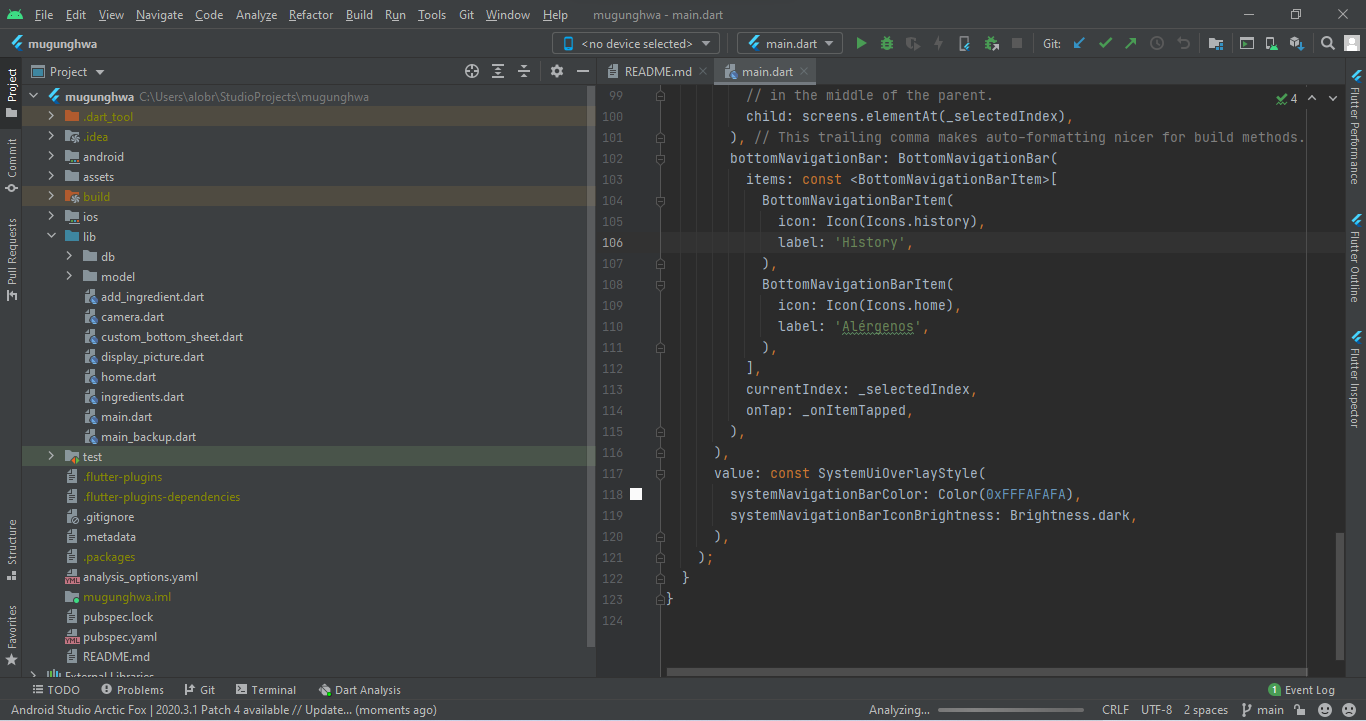
\includegraphics[width=\textwidth]{Figures/android-studio-screen.png}
  \caption{%
    Android Studio's user interface
  }
  \label{fig:android-studio-screen}
\end{figure}

It was still used occasionally because it offers way more Android-specific functions than our Visual Studio Code configuration. For example, it was used to create Android virtual devices (AVDs) for testing purposes.

\section{Version control}

In this section we will briefly describe the tools used to maintain a version control of the project source files and documentation.

\subsection{Git}

For efficiently keeping track of any changes made in the project code and documentation files we utilized Git \cite{noauthor_git_2021}. Git is a free and open-source version control software whose main purpose is registering any changes made on the project files, allowing to coordinate and synchronize the work across members of a team that are working on the same code. Git's logotype is shown in Figure \ref{fig:git}.

\begin{figure}[h]
  \centering
  
\includegraphics[width=0.5\textwidth]{Figures/git-logo.png}
  \caption{%
    Git's logotype
  }
  \label{fig:git}
\end{figure}

Even though the team is solely composed of one member, Git has been used to rollback to previous versions whenever needed, as well as to easily share any modifications with the project's director. It was also chosen because of the multiple integrations available with other tools in the stack such as Visual Studio Code or Overleaf. 

Git is also a distributed system, which means that the complete codebase (the files generated by the version control) is stored on the user computer instead of only on the server like in centralized client-server systems like such as Subversion \cite{noauthor_apache_nodate} or CVS \cite{noauthor_cvs_nodate}. Figure \ref{fig:git-repo} shows the repository structure and the files generated by Git in Git Bash, a CLI tool provided by the default installation.

\begin{figure}[h]
  \centering
  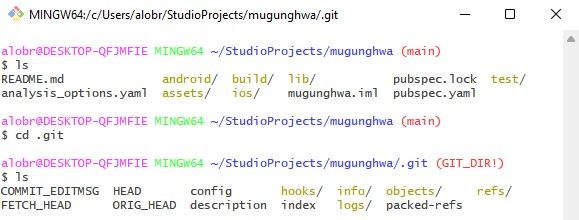
\includegraphics[width=0.75\textwidth]{Figures/git-repo.png}
  \caption{%
    Repository and files generated by Git
  }
  \label{fig:git-repo}
\end{figure}

Despite being a decentralized system, we also made use of a centralized platform for hosting our Git repository while having access to several additional features such as issue tracking, Kanban boards, \textit{wikis}, etc. This centralized hosting service is GitHub.

\subsection{GitHub}

GitHub \cite{noauthor_githubcom_2021} is a platform dedicated to provide hosting and version control services using Git for the source code of any software project. It was founded in 2008 and in 2018 it was acquired by Microsoft, which was already hosting over 4.500 of its projects on the platform. The projects stored in GitHub servers are typically public and available for everyone, as it is mainly a platform dedicated for open-source and collaborative projects. However, it also offers the possibility to open private repositories, first as a paid feature but available for free users too since April 2020. Figure \ref{fig:github-logo} shows GitHub's logotype.

\begin{figure}[h]
  \centering
  
\includegraphics[width=0.5\textwidth]{Figures/github-logo.png}
  \caption{%
    GitHub's logotype
  }
  \label{fig:github-logo}
\end{figure}

GitHub offers a wide array of functionalities that extend the basic Git usage, including \textit{wikis}, web pages, graphs and chart views for repository statistics, social features such as followers or stars, Kanban boards and even a cloud IDE based on Visual Studio Code. Out of these functionalities, Kanban boards and issue tracking were used extensively as explained in Chapter \ref{chapter4}. Besides, the platform was used to communicate issues in other pertinent repositories such as the Flutter one\footnote{Available at: \url{github.com/flutter/flutter}}, which is the 15th top repository by number of stars \cite{noauthor_repositories_nodate}. A screenshot of the GitHub repository used for hosting the code of the mobile application can be seen on Figure \ref{fig:github-repo}.

\begin{figure}[h]
  \centering
  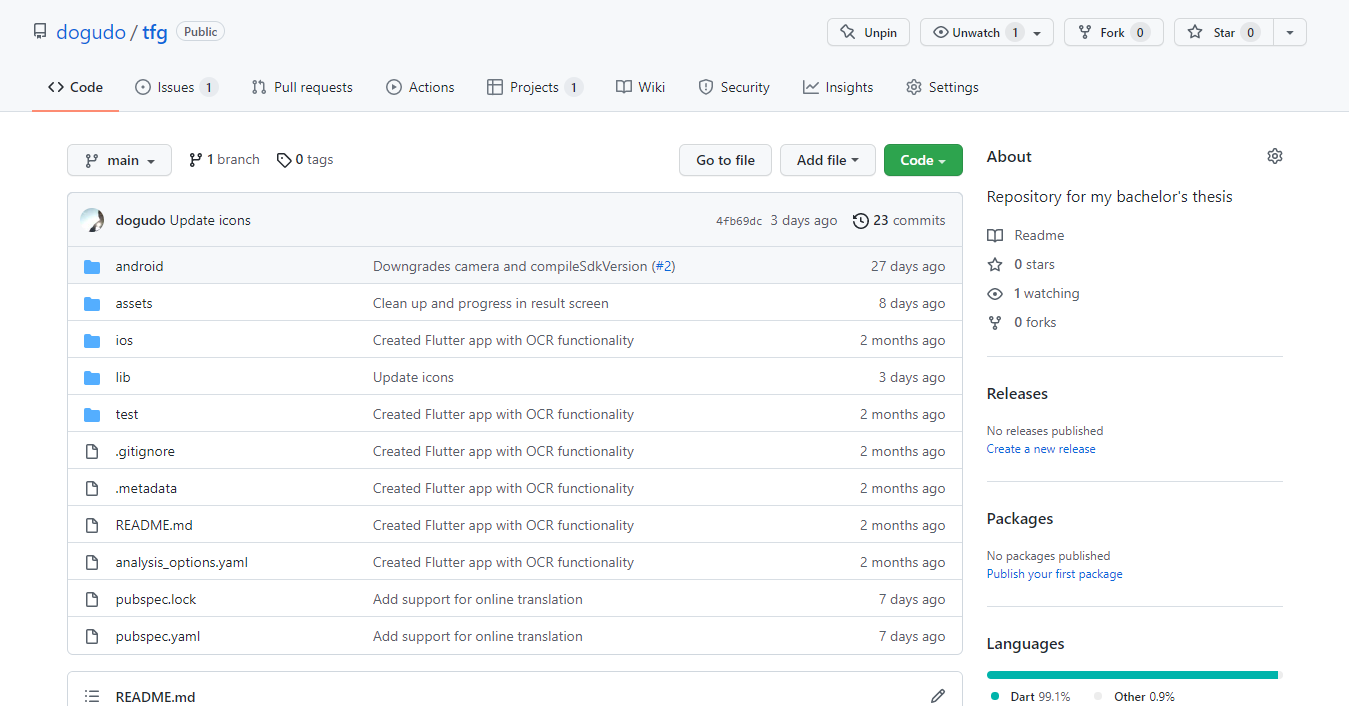
\includegraphics[width=\textwidth]{Figures/github-repo.png}
  \caption{%
    This project's repository hosted in GitHub
  }
  \label{fig:github-repo}
\end{figure}

For this project, two separate GitHub repositories were used. These are publicly available at the following locations:

\begin{itemize}
\item \texttt{tfg}, including the source files, database and other assets for the mobile application, is available at \url{github.com/dogudo/tfg}.
\item \texttt{tfg-report}, including the \LaTeX code of this report, is available at \url{github.com/dogudo/tfg-report}.
\end{itemize}

\section{Documentation}

In this section we will describe the tools that were used to compile, compose and write the documentation provided for the project, such as this report along with the charts and diagrams.

\subsection{\LaTeX}

\LaTeX\ \cite{noauthor_latex_nodate} is a high-quality typesetting ant text composing language, particularly oriented to the production of academic documents. As such, it has been widely adopted by the scientific community since its initial release back in 1984 and constitutes a de facto standard. It's logotype can be seen in Figure \ref{fig:latex}.

\begin{figure}[h]
  \centering
  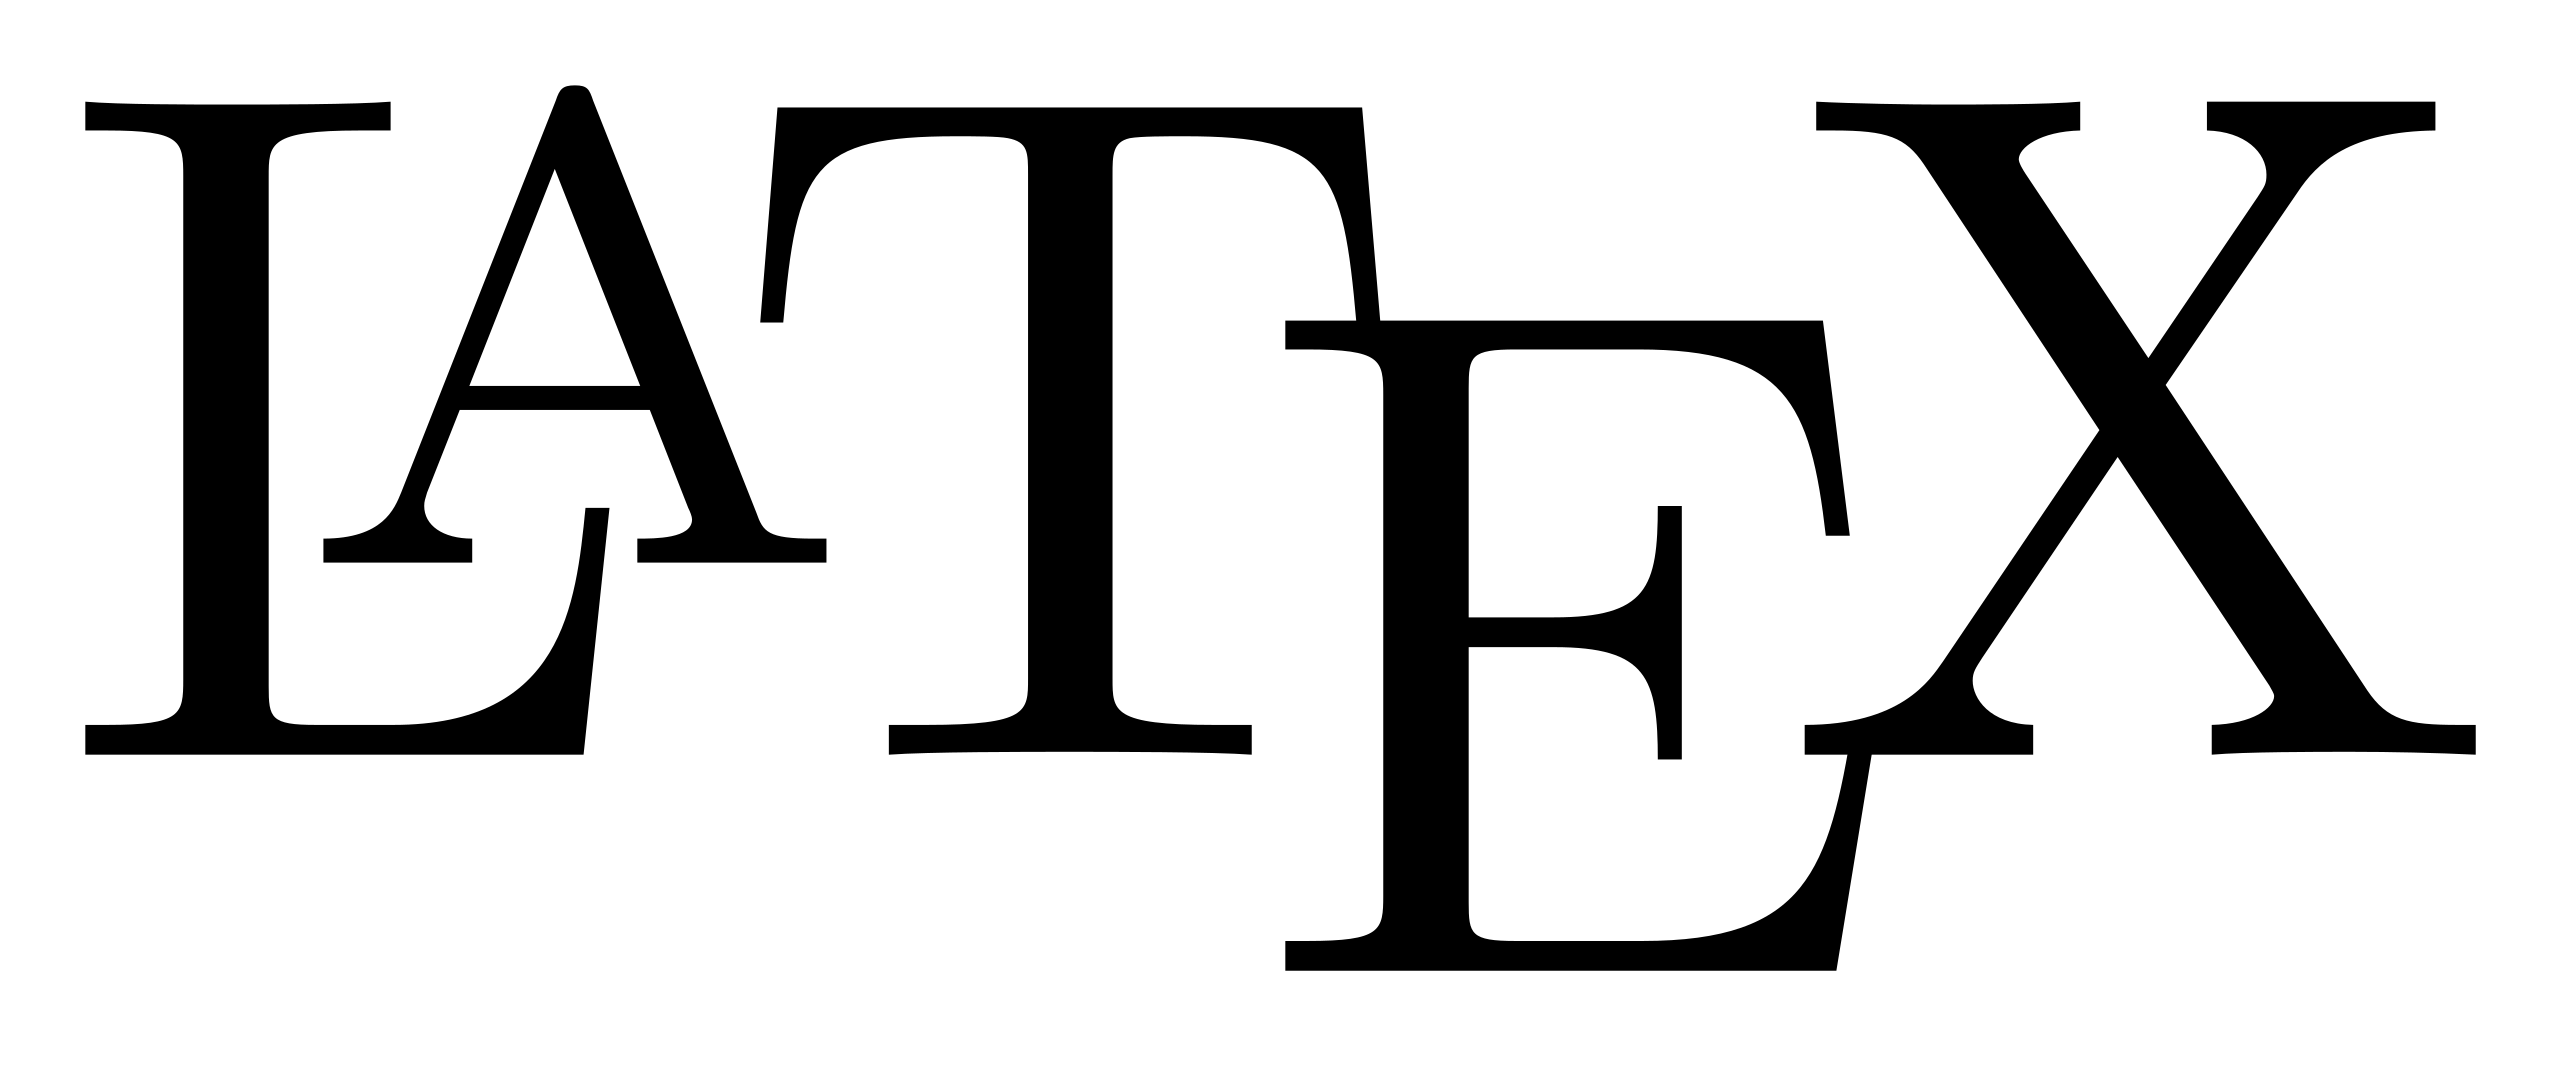
\includegraphics[width=0.5\textwidth]{Figures/latex.png}
  \caption{
    Latex's logotype.
  }
  \label{fig:latex}
\end{figure}

\LaTeX\ supports a great amount of plugins and commands to extend the base language and facilitate some functionalities such as including images, captions, text in non-Latin like \textit{hangeul}, import PDF pages from other documents, rotate figures, etc. In Listing \ref{lst:latex} we can see an example of the \LaTeX\ code needed to output both the previous figure and this paragraph.

\begin{code}
\begin{minted}[
breaklines,
frame=lines,
framesep=2mm,
baselinestretch=1.2,
fontsize=\footnotesize,
linenos
]{tex}
\begin{figure}[h]
  \centering
  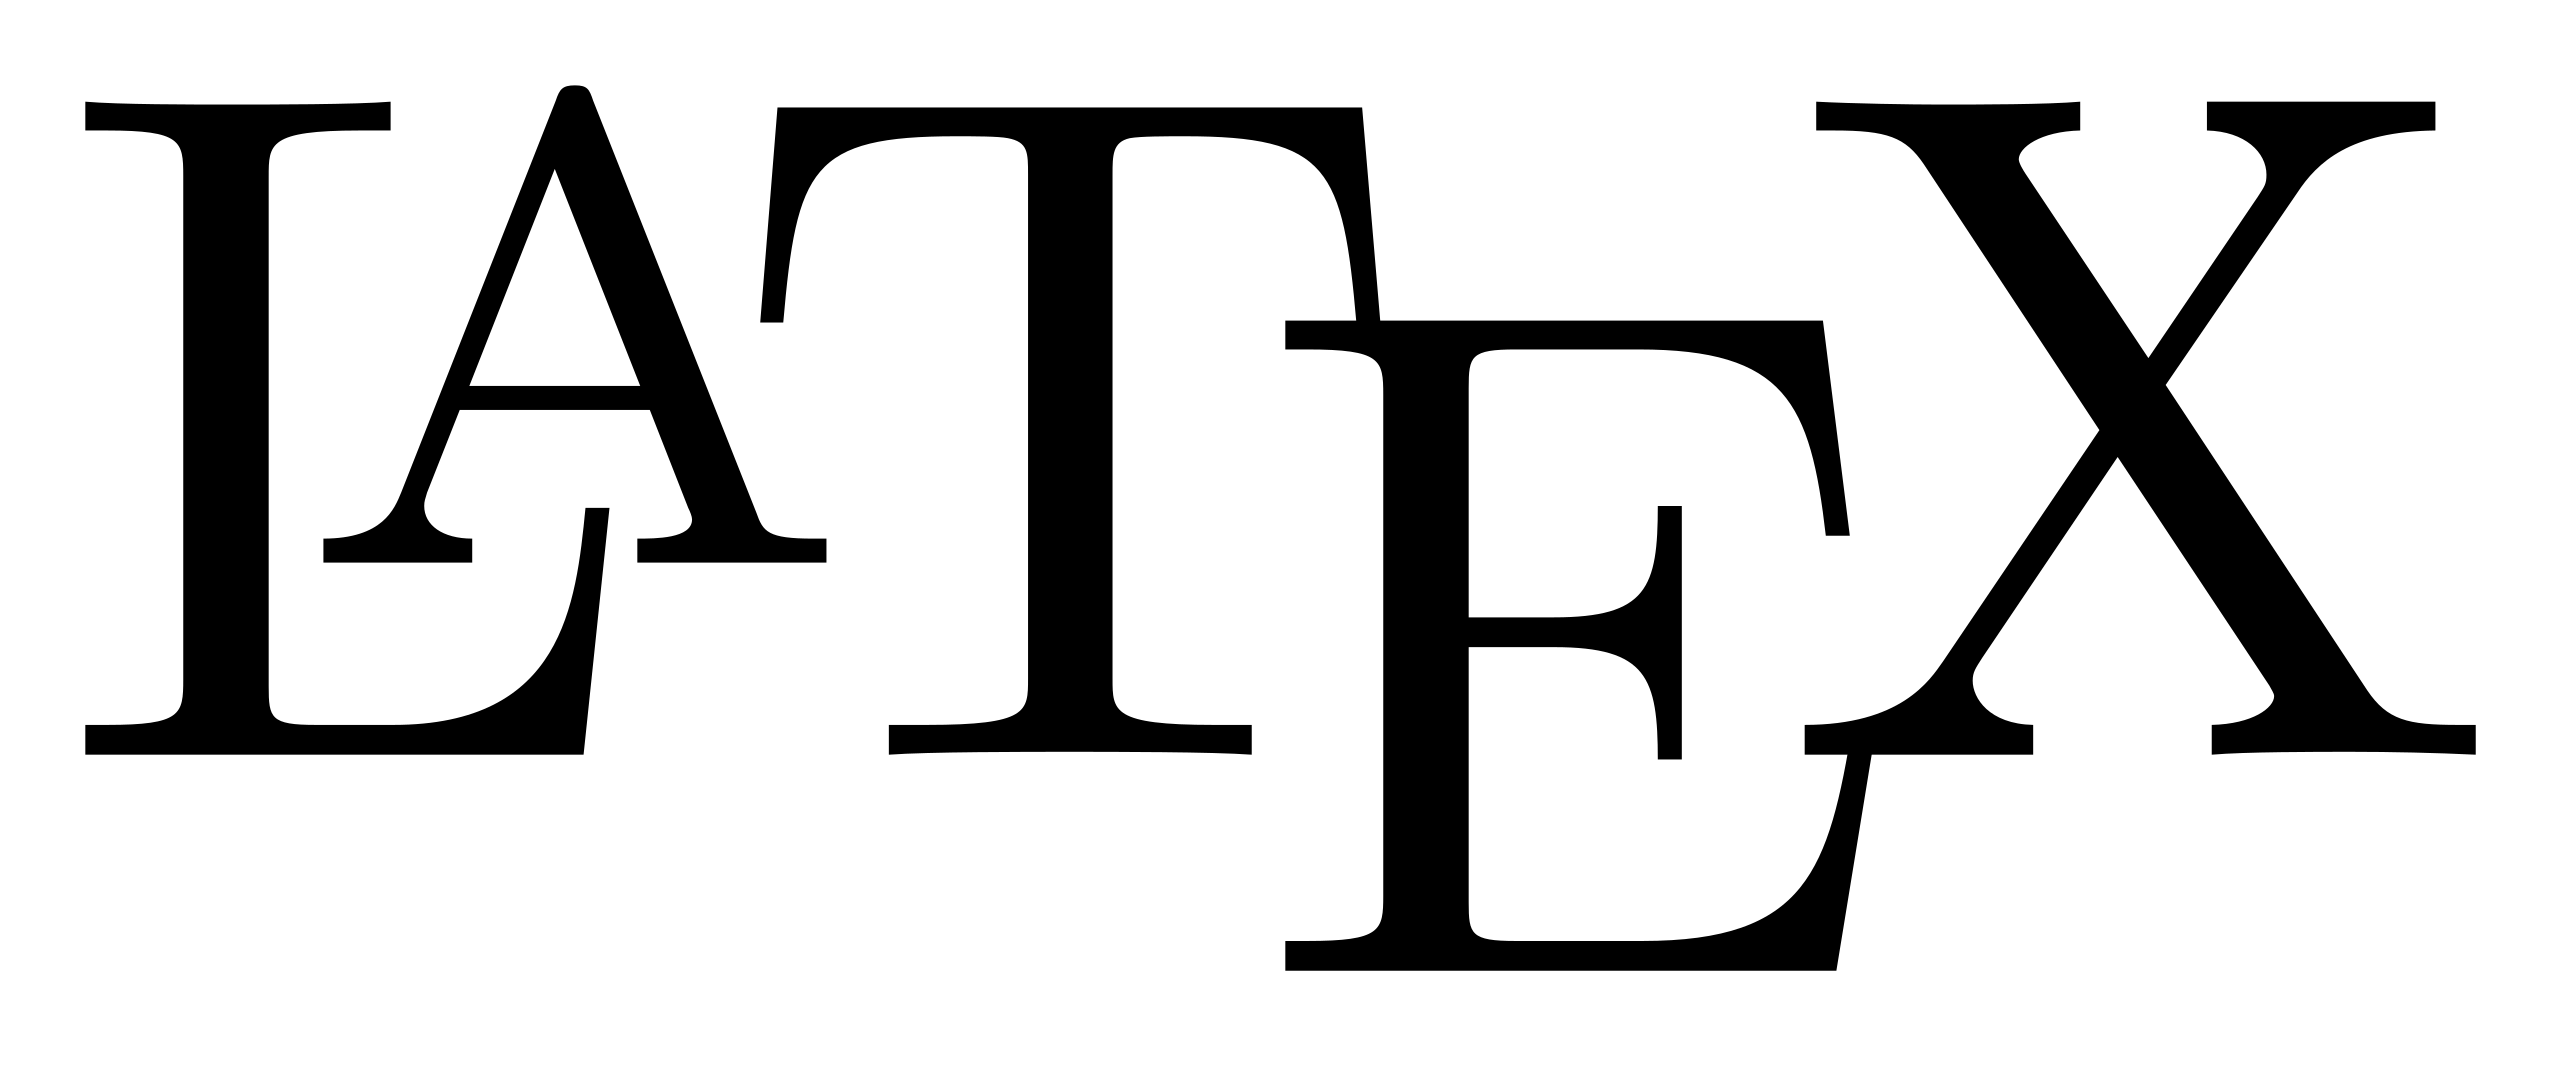
\includegraphics[width=0.5\textwidth]{Figures/latex.png}
  \caption{
    Latex's logotype.
  }
  \label{fig:latex}
\end{figure}

\LaTeX\ supports a great amount of plugins and commands to extend the base language and facilitate some functionalities such as including images, captions, text in non-Latin like \textit{hangeul}, import PDF pages from other documents, rotate figures, etc. In this project, it was the typesetting language of choice to compose this document. Figure \ref{lst:latex} shows an example of the \LaTeX\ code needed to output this paragraph.
\end{minted}
\caption{Example of \LaTeX\ code}
\label{lst:latex}
\end{code}

One of the main advantages of \LaTeX\ is that it has a large community and there are many templates readily available, which allows the user to focus on the writing task without having to worry about the structure and format of the document.

For this report we used a modified version of the \texttt{latex-mimosis} template by Bastian Rieck \cite{rieck_latex-mimosis_2022}, which is designed for typesetting thesis-like documents and is publicly hosted on a GitHub repository\footnote{Available at: \url{github.com/Pseudomanifold/latex-mimosis}}.

\subsection{Overleaf}

\subsection{Zotero}

\subsection{Draw.io}

\subsection{Microsoft Project}